\documentclass[conference]{IEEEtran}
\IEEEoverridecommandlockouts
% The preceding line is only needed to identify funding in the first footnote. If that is unneeded, please comment it out.
\usepackage{cite}
\usepackage{amsmath,amssymb,amsfonts}
\usepackage{algorithmic}
\usepackage{graphicx}
\usepackage{textcomp}
\usepackage[table]{xcolor}
\usepackage{listings}
\usepackage{booktabs}
\usepackage{numprint}
\usepackage[flushleft]{threeparttable}
\usepackage{tablefootnote}
\graphicspath{ {./figures/} }

\begin{document}

\title{Image Text Matching and Deep Reinforcement Learning Coursework Report}

\author{\IEEEauthorblockN{Liyou Zhou}
    \IEEEauthorblockA{\textit{Department of Computer Science} \\
        \textit{University of Lincoln}\\
        Lincoln, UK \\
        https://orcid.org/0009-0005-9491-9003}
}

\maketitle

\begin{abstract}
    Lorem ipsum dolor sit amet, consectetur adipiscing elit
\end{abstract}

\begin{IEEEkeywords}
    Image text matching, Vision Transformers, Deep Reinforcement Learning
\end{IEEEkeywords}


\section{Introduction}

Machine learning methods is revolutionizing the field of artificial intelligence. It has been applied to a wide range of tasks, from image recognition, natural language processing, to reinforcement learning.

In this coursework, we will explore two different machine learning tasks: image text matching and deep reinforcement learning.

For image text matching, image is encoded with convolution neural network or vision transformers. Text is encoded with a transformer. The embeddings are then combined to train a classifier to predict the relationship between the image and the text.

For deep reinforcement learning task, we will use the Mario game environment. The agent is trained to play the game using three different reinforcement learning algorithms: Deep Q-Learning, Advantage Actor Critic, and Proximal Policy Optimization.

\section{Background}

\subsection{Convolutions neural networks}

CNN has been the dominant architecture for image classification tasks. ResNet, proposed in \cite{heDeepResidualLearning2015} in 2015, achieved state-of-the-art performance on the ImageNet dataset. It introduced the concept of residual blocks, which allows the network to be trained deeper without the vanishing gradient problem. \textbf{Big Transfer} (BiT) - Based on ResNet\cite{heDeepResidualLearning2015}, is a training regime proposed in \cite{kolesnikovBigTransferBiT2020} that achieves improved performance on a number of image classification benchmarks via transfer learning. Proposed in \cite{liuConvNet2020s2022}, \textbf{ConvNeXt} is a pure convolutional network also based on ResNet but incorporates several design element of ViT.

\subsection{Vision Transformers}

Vision transformers is a relatively new architecture for image classification tasks. Transformers were originally designed for natural language processing tasks \cite{vaswaniAttentionAllYou2023}. \cite{dosovitskiyImageWorth16x162021} adapts the use of transformers for image inputs by dividing the image into patches and applying the attention modules to the patches. This architecture quickly surpassed CNN in performance on image classification task\cite{PapersCodeImageNet}.

\subsection{Language Representation Model}

Transformers \cite{vaswaniAttentionAllYou2023} haven been shown to be effective in encoding text data. \textbf{BERT} \cite{devlinBERTPretrainingDeep2019} is a text encoder trained on large corpus of text data from the internet. The resultant language representation can be used as input to a wide range of downstream tasks such as question and answering, text classification, and text generation. It has been shown in \cite{brownLanguageModelsAre2020} that these models can be fined tuned with relatively small sample of data to specific tasks.

\subsection{Deep Reinforcement Learning}

In solving learning task with complex and continuous state space, deep reinforcement learning algorithms has been shown to be effective. They are a class of algorithms that combines the conventional value-based or policy-based update algorithms with deep neural networks and trained with back-propagation.

\textbf{Deep Q-Learning} (DQN) is proposed in \cite{mnihPlayingAtariDeep2013} it includes several improvements on top of conventional Q-Learning:

\begin{itemize}
    \item CNN as state space encoder from image inputs.
    \item Neural network as a Q value function.
    \item Experience Relay buffer to store and sample experiences. This improves sample efficiency as each experience can be used in multiple weight updates.
\end{itemize}

\textbf{Advantage Actor Critic} (A2C) - Outlined by \cite{plaatDeepReinforcementLearning2022} employs the use of a critic to estimate how much better a particular action is compared to the expectation of a state. The actor then uses this information to update the policy.

\textbf{Proximal Policy Optimization} \cite{schulmanProximalPolicyOptimization2017} proposes a new class of policy based gradient methods for RL that alternative between sampling data from environment and optimizing the objective function. It further improves the sample efficiency by performing multiple epochs of optimization on the same batch of data.

\section{Image Text Matching Methodology}

\subsection{Image Encoder}

A number of image encoder has been added to the code for evaluation:

\begin{enumerate}
    \item Big Transfer (BiT) - Pre-trained CNN
    \item ConvNeXt - Pre-trained CNN
    \item ViT - Pre-trained Vision Transformer
    \item Vanilla Vision Transformers - Vision Transformer with no pre-training
\end{enumerate}

A comparison of standard benchmark scores of the pre-trained encoders can be seen in Table \ref{tab:image-encoder-comparison}. All these encoders are trained on the Image text matching task for 10 epochs and the losses and accuracy are plotted against the baseline in Figure \ref{fig:image_encoder_loss_and_accuracy}. BiT Model was able to achieve the highest training accuracy of 88.6\% followed by ConvNeXt at 83.6\% and ViT at 82.3\%. The vanilla Vision Transformer and the baseline CNN model required training from scratch and were not able to achieve the same level of accuracy as the pre-trained models.

\begin{table}
    \centering
    \caption{Image Encoder Comparison}
    \begin{tabular}{| p{1.2cm} | c | c | p{1.2cm} | p{1.2cm} |}
        \toprule
        Model & Variant & Pre-training & Parameters\linebreak (Million) & Accuracy\linebreak (\%) \tablefootnote{Top 1 accuracy on ImageNet} \\
        \midrule
        BiT & ResNet-101 & ImageNet-21k & ~40 & 87.5 \\
        \midrule
        ConvNeXt & Base & ImageNet & ~89 & 85.3 \\
        \midrule
        ViT & b32 & ImageNet-21k & ~88 & 81.3 \\
        \bottomrule
    \end{tabular}
    \label{tab:image-encoder-comparison}
\end{table}

\begin{figure}
    \centering
    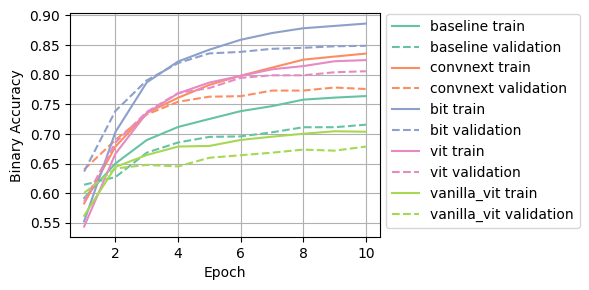
\includegraphics[width=0.49\textwidth]{image_encoder_loss_and_accuracy.png}
    \caption{Comparison of training and validation accuracy of the model with different image encoders. Trained for 10 epochs, fine tuning disabled. The dashed lines are valuation scores while the solid lines are training scores.}
    \label{fig:image_encoder_loss_and_accuracy}
\end{figure}

\subsection{Data Augmentation}

Image data is augmented to increase the training samples and improve the generalization of the model. The image input is randomly flipped, rotated, and zoomed during training.

\subsection{Text Encoder}

Instead of using directly the provided embeddings, 2 text encoders are added to the code for evaluation:

\begin{enumerate}
    \item BERT - Pre-trained transformer
    \item Vanilla Transformer - Transformer with no pre-training, trained from scratch with the rest of the model.
\end{enumerate}

Due to the constraint of the compute resources, only small version of BERT is used. Fig~\ref{fig:text_encoder_comparison} shows the comparison of all 3 encoders. The text embeddings provided in the task outperformed the transformer models.

\begin{figure}
    \centering
    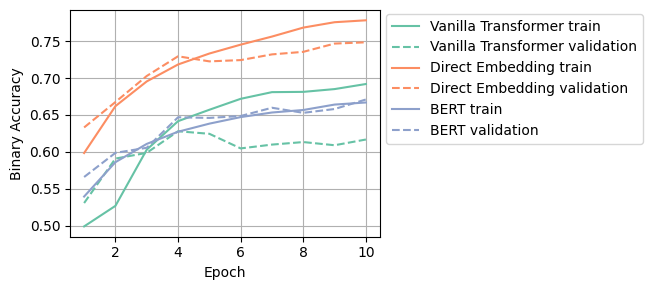
\includegraphics[width=0.49\textwidth]{text_encoder_comparison.png}
    \caption{Comparison of training and validation accuracy of the model with different text encoders}
    \label{fig:text_encoder_comparison}
\end{figure}

\subsection{Classifier}

The baseline classifier connects directly from the embeddings to the output classification. This only allow linear relationships between the embeddings and the output. To model more complex non-linear relationships, the classifier is extended to include a few hidden layers.

An attention layer is added to the classifier just after concatenating the text and image embeddings. This extracts information about each pair of elements in the embeddings and allows the model to learn better the relationship between the image and the text. Fig.~\ref{fig:classifier_comparison} shows the comparison of accuracy curve during training for the baseline direct classifier, adding hidden layers, and adding attention layer. The model with the attention layer achieved the highest accuracy of 94.3\% on the training set and 85.6\% on the validation set. It is notable that there is a large disparity between training and validation accuracy for the attention classifier. This suggests that the model is over-fitting to the training data.

\begin{figure}
    \centering
    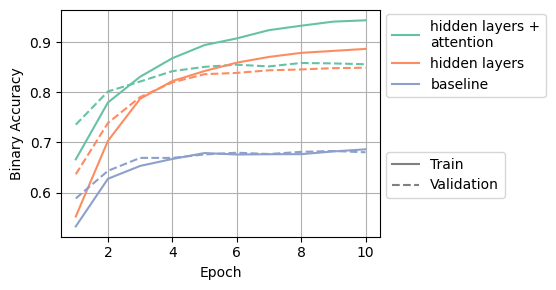
\includegraphics[width=0.49\textwidth]{classifier_comparison.png}
    \caption{Comparison of training and validation accuracy of the model with different classifiers}
    \label{fig:classifier_comparison}
\end{figure}

\section{Image Text Matching Results}

Taking the best performing modifications from the previous section, we train a model with BiT image encoding, direct text embedding from the task, and the classifier with attention layer. The model is trained until the validation accuracy stops improving. The training and validation accuracy curve is shown in Fig.~\ref{fig:final_model_accuracy}. The model achieved a training accuracy of 94.3\% and a validation accuracy of 85.6\%.



\section{Reinforcement Learning Methodology}

\subsection{Reinforcement Learning Algorithms}

3 Algorithms are tested:

\begin{enumerate}
    \item Deep Q-Learning (DQN) - value based method
    \item Advantage Actor Critic (A2C) - policy based actor critic architecture with experience replay.
    \item Proximal Policy Optimization (PPO) - policy based actor critic architecture with more effective experience replay and weights update.
\end{enumerate}

\subsection{State-action space reduction}

Mario game has a large sate-action space. For the learning algorithm to fully explore the space and learn a robust policy, the computational cost quickly becomes intractable. Hence a number of optimization is done to reduce the state-action space:

\begin{itemize}
    \item Image down-sampling - The image input is down-sampled to reduce the number of pixels to 64x64.
    \item Grey scaling - The image is converted to grey scale to reduce the number of channels.
    \item Reduce Action space: The action space is reduced to 4 actions: move right, jump, jump right, no op.
    \item Skip frames: Action is only applied every 4 frames of the game. The action is repeated for the skipped frames.
\end{itemize}

\subsection{Temporal Context}

Sometime it is important for the agent to understand the temporal context of the game. For example, the optimal action for Mario when a Goomba is moving towards him is different from when Goomba is moving away. The view of the game is completely identical if only looking at the single frame at a time.

To address this, 4 most recent frames are concatenated together to form the state input to the agent.

\subsection{Computer resource optimization}

To speed up the training process, the following optimization is done:
\begin{enumerate}
    \item Early termination - It is observed that the agent often gets stuck at a particular state and unable to advance to the right. Hence a custom wrapper is written for the environment so that the episode is terminated quickly in that situation.
    \item Parallelization - Multiple instances of the environment are run in parallel. Each environment is initialized with a different random seed. Agent is deployed on each instance and the experience is collected in parallel. Then policy/value update is done in a batch on the collected experience. This allows efficient use of the multi-core CPU and GPU resources.
\end{enumerate}

\subsection{Reward Shaping}

In the environment the reward is clipped to [-15, 15], then in the baseline implementation of the task, it is further clipped to [-1, 1]. \cite{vanhasseltLearningValuesMany2016} suggest that the learning algorithms are not reward scale invariant. Clipping makes the reward signal sparse and the agent has to explore a lot to find the optimal policy. Hence appropriate scale of the reward is important.

\section{Reinforcement Learning Results}

\section{Conclusion}



\bibliographystyle{IEEEtran}
\bibliography{IEEEabrv,AML.bib}

\end{document}
